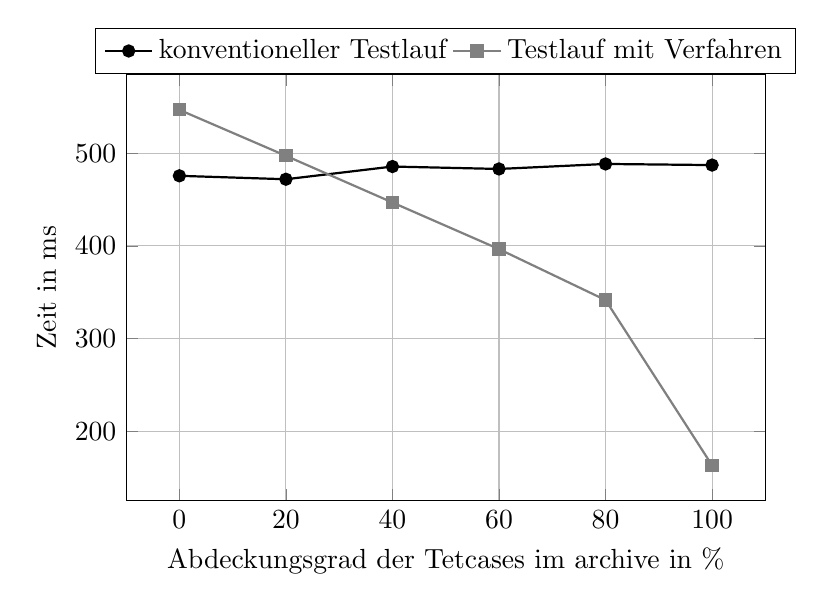
\begin{tikzpicture}
    \begin{axis}[
        width=0.8\textwidth,
        height=7cm,
        xlabel={Abdeckungsgrad der Tetcases im archive in \%},
        ylabel={Zeit in ms},
        grid=major,
        legend style={
            at={(0.5,1.0)},
            anchor=south,
            legend columns=2
        }
    ]
    \addplot[
        thick,
        mark=*,
    ] coordinates {
        (0, 475.6)
        (20, 471.9)
        (40, 485.6)
        (60, 483.0)
        (80, 488.4)
        (100, 487.2)
    };
    \addlegendentry{konventioneller Testlauf}
    \addplot[
        thick,
        mark=square*,
        gray!100,
    ] coordinates {
        (0, 546.8)
        (20, 497.2)
        (40, 446.8)
        (60, 396.5)
        (80, 341.5)
        (100, 163.1)
    };
    \addlegendentry{Testlauf mit Verfahren}
    \end{axis}
\end{tikzpicture}
